\chapter{Design}\label{ch:Design}

This chapter presents the architectural design of the electricity demand forecasting system. It describes the overall pipeline, data acquisition strategy, feature engineering approach, model selection rationale, and the design of the PPSO-based hyperparameter optimisation process.


\section{System Architecture Overview}

The forecasting system is designed as a modular, end-to-end machine learning pipeline comprising six sequential stages: configuration loading, data acquisition, preprocessing and feature engineering, train/test splitting, model training and hyperparameter tuning, and evaluation with visualisation. Figure~\ref{fig:pipeline_flowchart} presents the high-level pipeline architecture.

\begin{figure}[H]
\centering
\begin{tikzpicture}[
    node distance=1.2cm and 1.5cm,
    block/.style={rectangle, draw, fill=blue!8, text width=10em, text centered, minimum height=2.8em, rounded corners=3pt, font=\small},
    decision/.style={diamond, draw, fill=orange!12, text width=6em, text centered, aspect=2.2, inner sep=1pt, font=\small},
    data/.style={rectangle, draw, fill=green!8, text width=9em, text centered, minimum height=2.5em, rounded corners=3pt, font=\small},
    arrow/.style={-{Stealth[length=2.5mm]}, thick}
]

% Nodes
\node[block] (config) {1. Load Configuration\\(\texttt{config.yaml})};
\node[data, below=of config] (weather) {Weather Data\\(Open-Meteo API)};
\node[data, right=2.5cm of weather] (demand) {Demand Data\\(EMA CSV)};
\node[block, below=1.0cm of $(weather)!0.5!(demand)$] (merge) {2. Merge \& Validate\\Data};
\node[block, below=of merge] (preprocess) {3. Feature Engineering\\(16 features)};
\node[block, below=of preprocess] (split) {4. Chronological\\Train/Test Split (80/20)};
\node[block, below left=1.2cm and 1.5cm of split] (train_std) {5a. Train Standard\\Models (LR, RF, XGB, CB)};
\node[block, below right=1.2cm and 1.5cm of split] (train_ppso) {5b. PPSO Optimise\\RF / XGB / CatBoost};
\node[block, below=1.0cm of $(train_std)!0.5!(train_ppso)$] (evaluate) {6. Evaluate All Models\\(6 Metrics)};
\node[data, below=of evaluate] (output) {Results: Leaderboard,\\Plots, Summary};

% Arrows
\draw[arrow] (config) -- (weather);
\draw[arrow] (config) -| (demand);
\draw[arrow] (weather) |- (merge);
\draw[arrow] (demand) |- (merge);
\draw[arrow] (merge) -- (preprocess);
\draw[arrow] (preprocess) -- (split);
\draw[arrow] (split) -| (train_std);
\draw[arrow] (split) -| (train_ppso);
\draw[arrow] (train_std) |- (evaluate);
\draw[arrow] (train_ppso) |- (evaluate);
\draw[arrow] (evaluate) -- (output);

\end{tikzpicture}
\caption{High-level architecture of the electricity demand forecasting pipeline.}
\label{fig:pipeline_flowchart}
\end{figure}

Each stage is implemented as an independent Python module, enabling modularity, testability, and ease of modification. A single YAML configuration file controls all pipeline parameters, from data paths and weather API coordinates to model hyperparameter bounds and output directories.


\section{Data Acquisition Design}\label{sec:data_design}

\subsection{Electricity Demand Data}

Daily electricity demand data for Singapore is obtained from the Energy Market Authority (EMA) \parencite{ema2025statistics}. The data is stored as a CSV file (\texttt{ema\_daily\_demand.csv}) with two columns: \texttt{date} (YYYY-MM-DD) and \texttt{demand\_mwh} (total daily demand in megawatt-hours). The dataset spans from January 2023 to December 2025, providing 1,096 daily observations.

\subsection{Weather Data}

Historical weather observations are retrieved programmatically from the Open-Meteo Archive API \parencite{openmeteo2025api}, which provides free access to reanalysis and station-interpolated meteorological data. The API is queried with Singapore's geographic coordinates (1.3521$^\circ$N, 103.8198$^\circ$E) to retrieve four daily weather variables:

\begin{table}[H]
\centering
\caption{Weather variables retrieved from Open-Meteo API.}
\label{tab:weather_vars}
\begin{tabular}{@{}lll@{}}
\toprule
\textbf{Variable} & \textbf{API Parameter} & \textbf{Unit} \\
\midrule
Mean temperature & \texttt{temperature\_2m\_mean} & $^\circ$C \\
Mean relative humidity & \texttt{relative\_humidity\_2m\_mean} & \% \\
Maximum wind speed & \texttt{wind\_speed\_10m\_max} & m/s \\
Cumulative solar radiation & \texttt{shortwave\_radiation\_sum} & W/m$^2$ \\
\bottomrule
\end{tabular}
\end{table}

\subsection{Data Integration}

The weather and demand datasets are merged on the \texttt{date} column using an inner join, ensuring that only dates with both weather observations and demand records are retained. After merging, the dataset is sorted chronologically and validated (minimum 31 rows required). The merged dataset contains 1,065 daily observations spanning February 2023 to December 2025.


\section{Feature Engineering Design}\label{sec:feature_design}

A total of 16 features are constructed from the raw data across four categories. Table~\ref{tab:feature_set} provides a complete description.

\begin{table}[H]
\centering
\caption{Complete feature set used for demand forecasting (16 features).}
\label{tab:feature_set}
\small
\begin{tabular}{@{}llll@{}}
\toprule
\textbf{Category} & \textbf{Feature} & \textbf{Type} & \textbf{Description} \\
\midrule
\multirow{4}{*}{Weather} 
  & \texttt{temperature} & Numeric & Daily mean temperature ($^\circ$C) \\
  & \texttt{humidity} & Numeric & Daily mean relative humidity (\%) \\
  & \texttt{wind\_speed} & Numeric & Daily max wind speed (m/s) \\
  & \texttt{solar\_radiation} & Numeric & Cumulative radiation (W/m$^2$) \\
\addlinespace
\multirow{2}{*}{Derived}
  & \texttt{cci} & Numeric & Comfort Climate Index (Eq.~\ref{eq:cci}) \\
  & \texttt{season} & Categorical & Season (1--4, derived from month) \\
\addlinespace
\multirow{4}{*}{Temporal}
  & \texttt{day\_of\_week} & Categorical & 0 (Mon) to 6 (Sun) \\
  & \texttt{month} & Categorical & 1--12 \\
  & \texttt{is\_weekend} & Binary & 1 if Saturday/Sunday \\
  & \texttt{is\_holiday} & Binary & 1 if Singapore public holiday \\
\addlinespace
\multirow{6}{*}{Autoregressive}
  & \texttt{demand\_lag\_1} & Numeric & Demand 1 day ago \\
  & \texttt{demand\_lag\_7} & Numeric & Demand 7 days ago \\
  & \texttt{demand\_rolling\_mean\_3} & Numeric & 3-day rolling mean demand \\
  & \texttt{demand\_rolling\_mean\_7} & Numeric & 7-day rolling mean demand \\
  & \texttt{demand\_rolling\_std\_3} & Numeric & 3-day rolling std of demand \\
  & \texttt{demand\_rolling\_std\_7} & Numeric & 7-day rolling std of demand \\
\bottomrule
\end{tabular}
\end{table}

\subsection{Rationale for Feature Categories}

\begin{itemize}
    \item \textbf{Weather features} provide the exogenous drivers of cooling demand. Temperature and humidity are expected to be the strongest weather predictors given Singapore's air-conditioning-dominated load profile.
    
    \item \textbf{Derived features}: The CCI captures the combined effect of temperature and humidity on thermal comfort (Equation~\ref{eq:cci}). The season variable provides a coarse temporal grouping that may capture monsoon-related demand patterns.
    
    \item \textbf{Temporal features} encode calendar effects. Weekend and holiday indicators capture the well-documented demand reduction on non-working days, while day-of-week and month allow the model to learn finer-grained periodic patterns.
    
    \item \textbf{Autoregressive features} incorporate demand history. Lag-1 captures the strong day-to-day autocorrelation of demand, while lag-7 captures weekly periodicity. Rolling means and standard deviations smooth out noise and provide information about recent demand trends and volatility.
\end{itemize}

The construction of lag and rolling features introduces missing values at the beginning of the time series (up to 7 days for lag-7, up to 7 days for rolling-7). These rows are dropped after feature engineering, resulting in the final dataset of 1,065 usable observations.


\section{Model Selection Rationale}

Eight model configurations were selected to provide a progression from simple to complex, and to enable a \emph{fair} assessment of hyperparameter optimisation:

\begin{enumerate}
    \item \textbf{Baseline (Lag-1)}: Predicts today's demand as yesterday's demand. Any useful model must beat this.

    \item \textbf{Linear Regression}: Serves as an interpretable baseline. Features are standardised using \texttt{StandardScaler} before fitting.
    
    \item \textbf{Random Forest (default)}: Captures non-linear relationships and interactions without requiring feature scaling. Provides feature importance via impurity reduction.
    
    \item \textbf{XGBoost (default)}: Sequential boosting with regularisation. Tests whether gradient boosting improves over bagging (RF).
    
    \item \textbf{CatBoost (default)}: Native categorical feature handling. Tests whether ordered boosting and target statistics improve over XGBoost for this dataset.
    
    \item \textbf{RF-PPSO, XGB-PPSO, and CatBoost-PPSO}: Each tree-based model with PPSO-optimised hyperparameters under an \emph{identical} optimisation budget (same swarm size, iteration limit, and time-series cross-validation fitness). Applying PPSO to all tunable models---rather than to CatBoost alone---ensures that the comparison isolates the intrinsic merit of each learning algorithm from the benefit of hyperparameter tuning, avoiding an unfair advantage for any single model.
\end{enumerate}

This progression allows us to isolate the contribution of each methodological improvement: non-linearity (LR $\to$ RF), sequential boosting (RF $\to$ XGBoost), categorical handling (XGBoost $\to$ CatBoost), and hyperparameter optimisation (each default model $\to$ its PPSO-tuned variant).


\section{PPSO Hyperparameter Tuning Design}\label{sec:ppso_design}

PPSO \parencite{ghasemi2019ppso} was chosen as the hyperparameter optimiser for three reasons. First, it is \emph{parameter-free}: unlike standard PSO, it requires no manual tuning of inertia weight or acceleration coefficients ($w$, $c_1$, $c_2$), because the phasor angle $\theta$ modulates the cognitive and social terms adaptively---this removes a layer of meta-tuning that would itself bias the comparison. Second, the periodic (sine/cosine) modulation of particle velocities provides a natural balance between global exploration and local exploitation, which suits the non-convex, expensive-to-evaluate objective landscape of hyperparameter search where each fitness evaluation requires several full model training runs. Third, the reference study \parencite{zhang2023catboostppso} demonstrated that PPSO outperformed standard PSO and other meta-heuristics when tuning CatBoost for short-term electricity consumption forecasting, making it a well-validated choice for this problem domain.

The PPSO optimiser is configured to search over a four-dimensional hyperparameter space per model (Table~\ref{tab:catboost_hyperparams} shows the CatBoost space; analogous spaces are defined for Random Forest---\texttt{n\_estimators}, \texttt{max\_depth}, \texttt{min\_samples\_split}, \texttt{min\_samples\_leaf}---and XGBoost---\texttt{n\_estimators}, \texttt{max\_depth}, \texttt{learning\_rate}, \texttt{reg\_lambda}). The design choices are as follows:

\begin{itemize}
    \item \textbf{Swarm size}: 15 particles. Balances exploration breadth with computational cost.
    \item \textbf{Maximum iterations}: 20 PPSO iterations. Each iteration evaluates all 15 particles.
    \item \textbf{Fitness function}: Mean RMSE from 3-fold \texttt{TimeSeriesSplit} cross-validation on the training set. Time-series splitting ensures that each validation fold contains only future data relative to its training fold, preventing temporal leakage.
    \item \textbf{Early stopping}: PPSO terminates if the global best fitness does not improve for 5 consecutive iterations. CatBoost also uses internal early stopping (20 rounds) within each cross-validation fold.
    \item \textbf{Velocity clamping}: Velocities are clamped using the phasor-modulated maximum velocity (Equation~\ref{eq:ppso_vmax}) to prevent particles from overshooting the search bounds.
\end{itemize}

\begin{figure}[H]
\centering
\begin{tikzpicture}[
    node distance=1.1cm,
    block/.style={rectangle, draw, fill=blue!8, text width=12em, text centered, minimum height=2.5em, rounded corners=3pt, font=\small},
    decision/.style={diamond, draw, fill=orange!12, text width=7em, text centered, aspect=2, inner sep=1pt, font=\small},
    arrow/.style={-{Stealth[length=2.5mm]}, thick}
]

\node[block] (init) {Initialise $N$ particles\\with random positions \& phases};
\node[block, below=of init] (eval) {For each particle:\\Train candidate model with\\3-fold TS cross-validation};
\node[block, below=of eval] (fitness) {Compute fitness =\\mean validation RMSE};
\node[block, below=of fitness] (update_pb) {Update personal best\\and global best};
\node[block, below=of update_pb] (ppso_update) {PPSO velocity, position,\\and phase angle update};
\node[decision, below=of ppso_update] (converge) {Converged or\\max iter?};
\node[block, below left=1.2cm and 0cm of converge] (final) {Train final model\\with best hyperparameters\\on full training set};

\draw[arrow] (init) -- (eval);
\draw[arrow] (eval) -- (fitness);
\draw[arrow] (fitness) -- (update_pb);
\draw[arrow] (update_pb) -- (ppso_update);
\draw[arrow] (ppso_update) -- (converge);
\draw[arrow] (converge) -- node[right, font=\small]{Yes} (final);
\draw[arrow] (converge.east) -- ++(1.8,0) |- node[near start, right, font=\small]{No} (eval.east);

\end{tikzpicture}
\caption{PPSO hyperparameter optimisation workflow (applied identically to Random Forest, XGBoost, and CatBoost).}
\label{fig:ppso_workflow}
\end{figure}


\section{Train/Test Split Strategy}

A chronological 80/20 split is employed: the first 852 observations form the training set, and the remaining 213 observations form the test set. Unlike random splitting, chronological splitting preserves the temporal ordering of the data and prevents future information from leaking into the training process. This is essential for time-series forecasting, where the model must generalise to unseen future dates.

\begin{table}[H]
\centering
\caption{Train/test split statistics.}
\label{tab:split_stats}
\begin{tabular}{@{}lrrr@{}}
\toprule
\textbf{Partition} & \textbf{Samples} & \textbf{Proportion} & \textbf{Date Range} \\
\midrule
Training set & 852 & 80\% & Feb 2023 -- Jun 2025 \\
Test set & 213 & 20\% & Jul 2025 -- Dec 2025 \\
\midrule
Total & 1{,}065 & 100\% & Feb 2023 -- Dec 2025 \\
\bottomrule
\end{tabular}
\end{table}


\section{Exploratory Data Analysis}

Before model training, exploratory data analysis (EDA) was conducted to understand the structure and relationships within the dataset.

\begin{figure}[H]
    \centering
    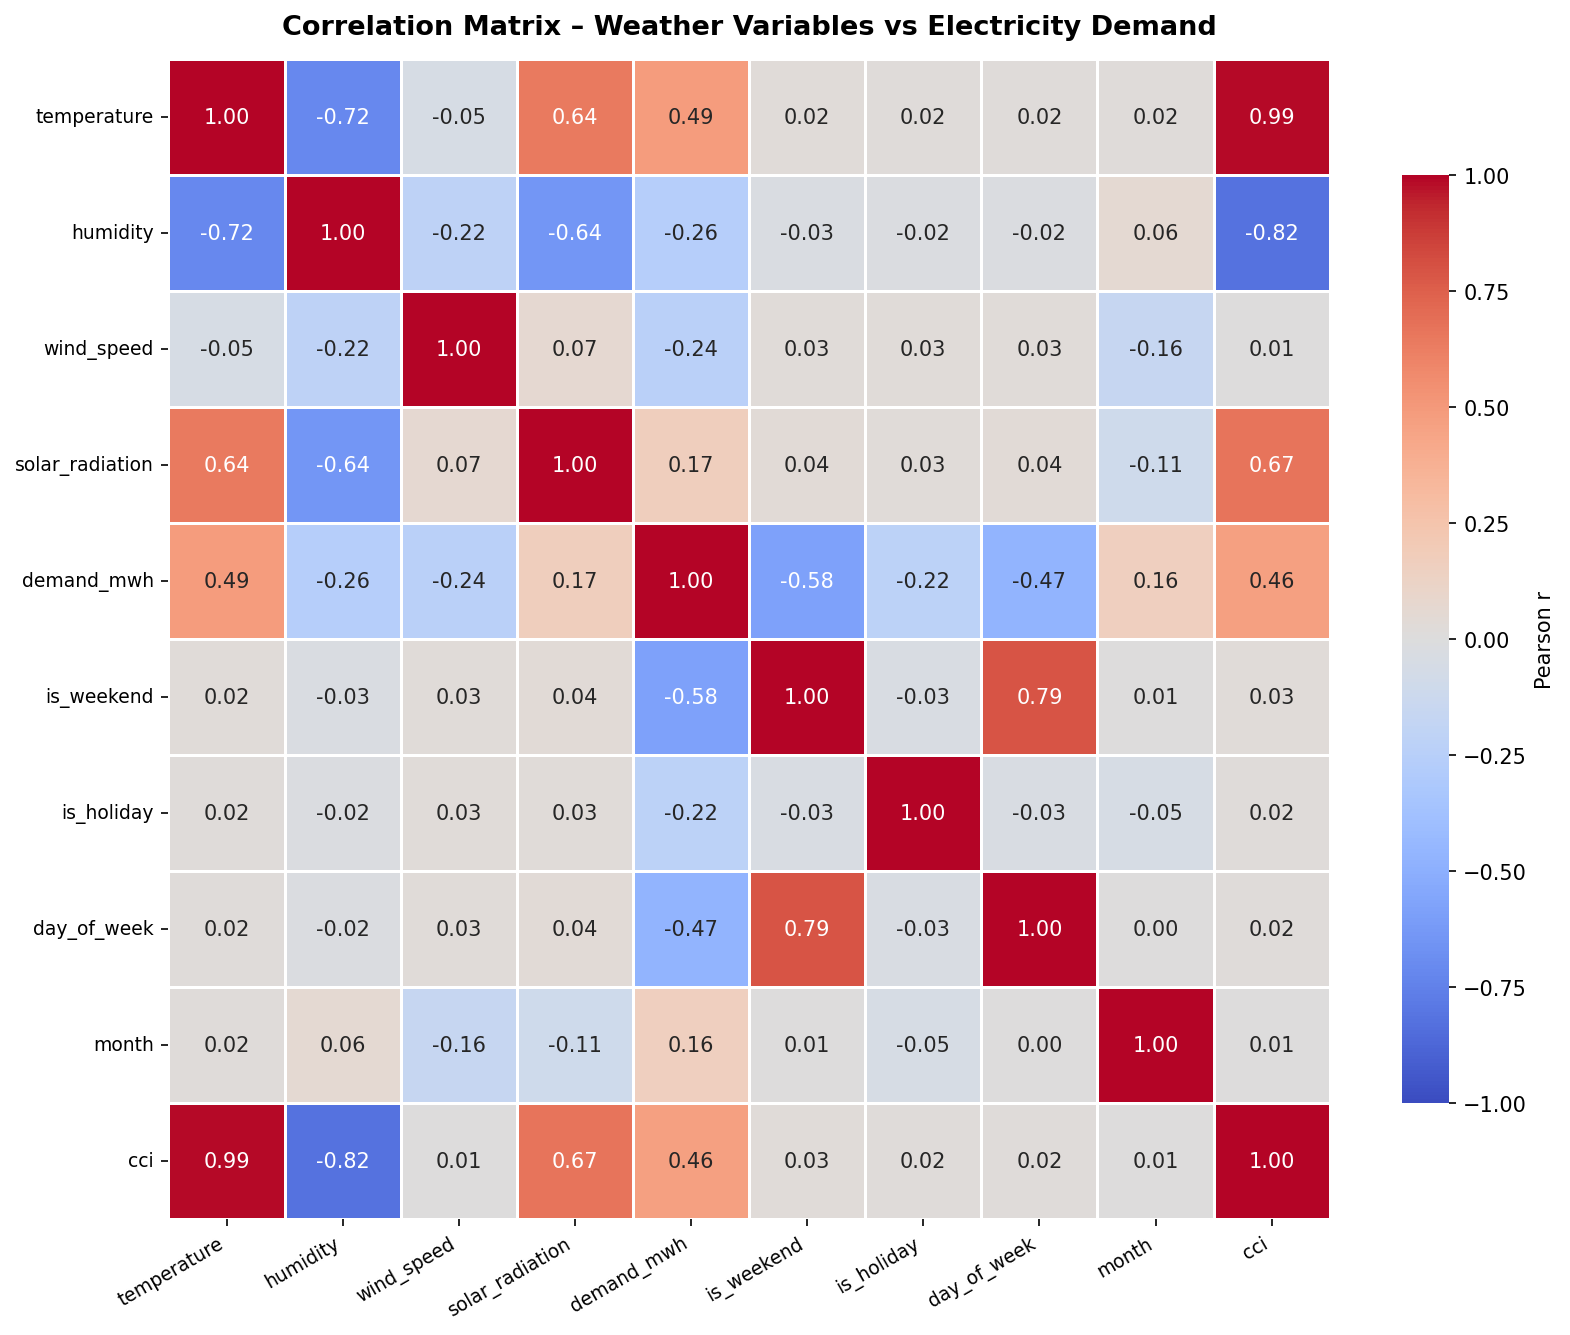
\includegraphics[width=0.85\textwidth]{design/images/eda_correlation_heatmap.png}
    \caption{Pearson correlation heatmap of all numeric features and the target variable (\texttt{demand\_mwh}). Lag-1 demand shows the strongest correlation with the target, followed by rolling mean features and temperature.}
    \label{fig:correlation_heatmap}
\end{figure}

\begin{figure}[H]
    \centering
    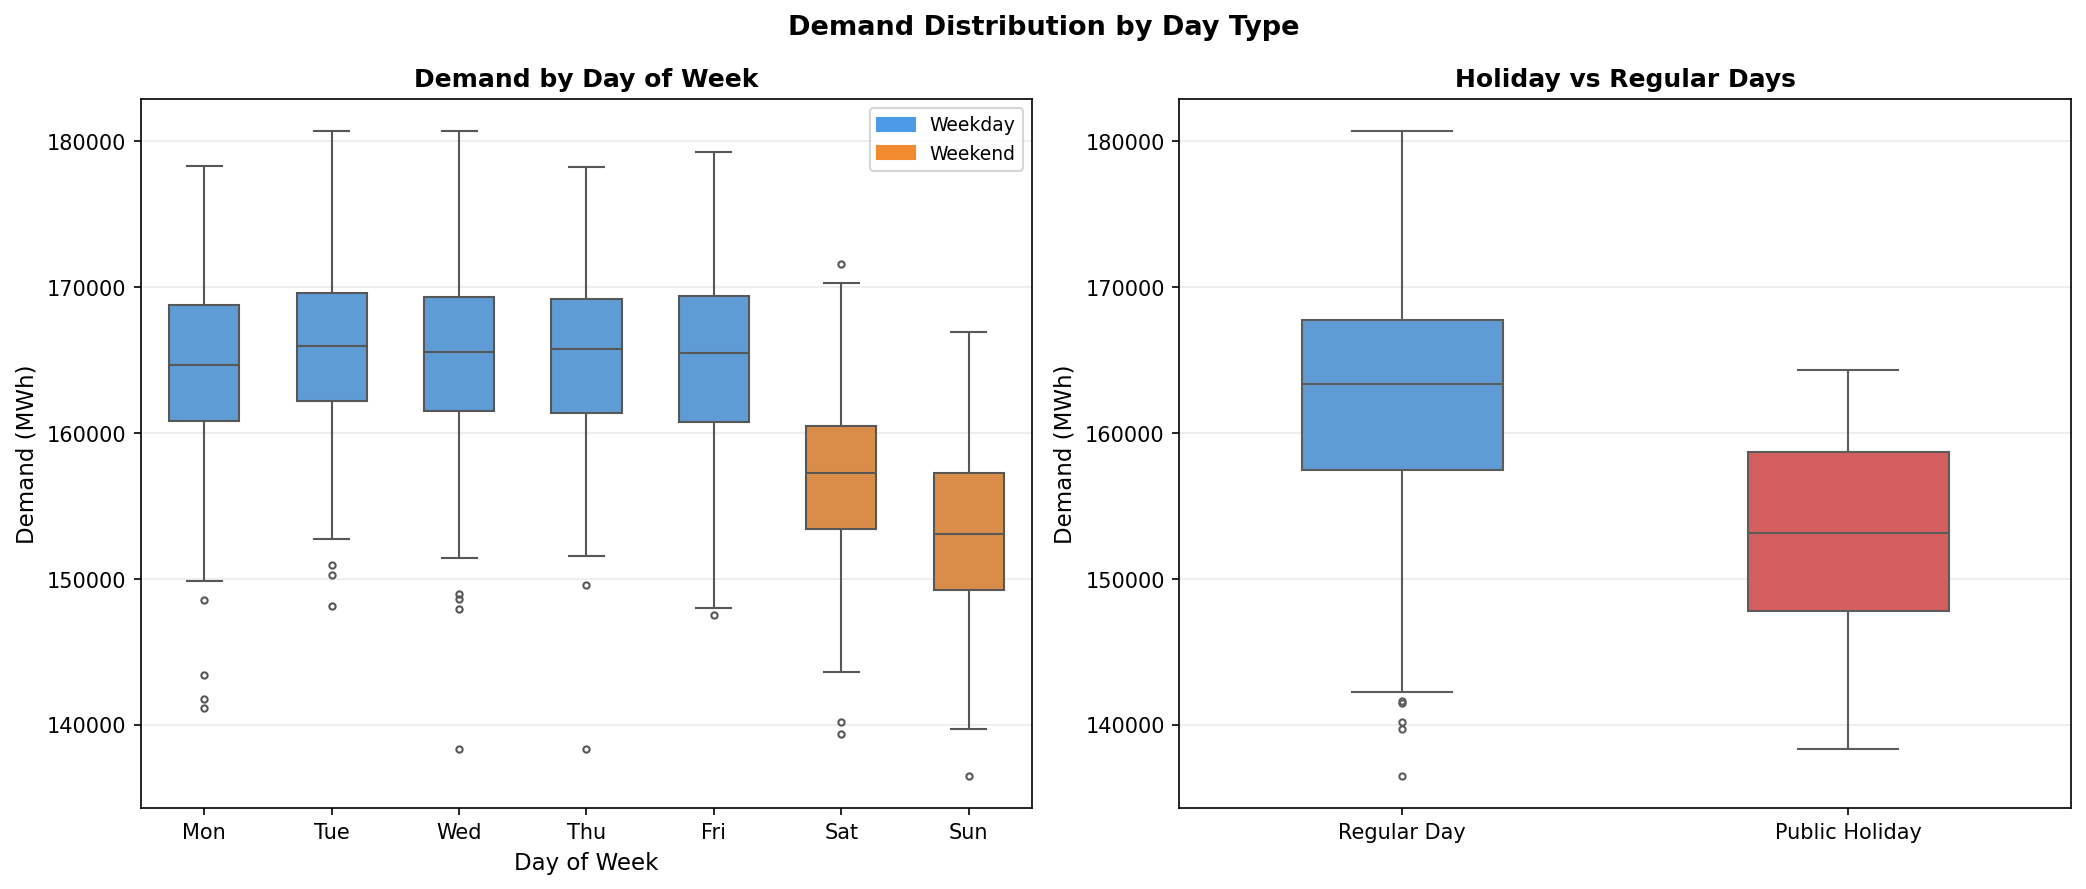
\includegraphics[width=0.85\textwidth]{design/images/eda_demand_by_daytype.png}
    \caption{Distribution of daily electricity demand by day type (weekday vs.\ weekend/holiday). Weekday demand is consistently higher, confirming the importance of temporal calendar features.}
    \label{fig:demand_daytype}
\end{figure}


\section{Conclusions}

This chapter has presented the design of a modular forecasting pipeline that integrates weather and demand data, constructs 16 engineered features across four categories, trains eight model configurations of progressively increasing complexity, and employs PPSO for automated hyperparameter tuning of every tree-based model under an identical optimisation budget, ensuring a fair comparison. The chronological train/test split ensures evaluation integrity. The following chapter describes the technical implementation of each component.
